% =====================================================================
%  DATA AND PREPROCESSING REPORT
%  MLE-AI-201 Machine Learning -- Final Project (bina.az sale dataset)
%
%  Self-contained: uses only standard LaTeX packages, no IEEEtran.cls.
%  Build:  tectonic report/data_report.tex
%     or:  pdflatex data_report.tex ; pdflatex data_report.tex
%
%  Every number in this document is produced by:
%     python explore.py --data data/bina_az_sale.csv --out reports/eda
%     python -m src.data_prep
% =====================================================================
\documentclass[10pt,twocolumn,a4paper]{article}

\usepackage[a4paper,top=0.75in,bottom=1.0in,left=0.68in,right=0.68in,columnsep=0.25in]{geometry}
\usepackage{mathptmx}
\usepackage[T1]{fontenc}
\usepackage[utf8]{inputenc}
\usepackage{graphicx}
\usepackage{amsmath,amssymb}
\usepackage{booktabs}
\usepackage{array}
\usepackage{titlesec}
\usepackage{caption}
\usepackage[hidelinks]{hyperref}
\usepackage{url}

\renewcommand{\thesection}{\Roman{section}}
\renewcommand{\thesubsection}{\Alph{subsection}}
\titleformat{\section}[block]{\centering\normalsize\scshape}{\thesection.}{0.5em}{}
\titleformat{\subsection}[block]{\normalsize\itshape}{\thesubsection.}{0.5em}{}
\titlespacing*{\section}{0pt}{1.4ex plus 1ex minus .2ex}{1ex}
\titlespacing*{\subsection}{0pt}{1.0ex plus 1ex minus .2ex}{0.6ex}

\newcommand{\abstractkw}[1]{\noindent\textbf{\textit{#1}}}
\captionsetup{font=small,labelsep=period}
\setlength{\parindent}{1em}
\graphicspath{{figures/}}

% =====================================================================
\begin{document}

\twocolumn[
  \begin{@twocolumnfalse}
  \begin{center}
    {\LARGE\bfseries From Scraped Adverts to a Model-Ready Table:\\
     Preparing the bina.az Property Dataset\par}
    \vspace{1.2em}
    {\large Team PegaSold\par}
    \vspace{0.5em}
    {\itshape MLE-AI-201 Machine Learning, AI Academy --- Cohort II\par}
    \vspace{1.4em}
  \end{center}
  \begin{quote}
    \small
    \abstractkw{Abstract---}%
    We describe how the raw bina.az property dataset was turned into a
    table suitable for machine learning. The raw file holds 100{,}775
    adverts across 51 columns, scraped repeatedly over six weeks. We
    found four problems that would each, on its own, have produced a
    model that looks excellent and is worthless: three columns that
    already contain the answer, 37{,}534 rows that are repeat sightings
    of adverts we had already seen, one column that silently mixes two
    units of measurement, and a set of columns where an empty cell means
    ``no'' rather than ``unknown''. We explain each problem, the evidence
    that it is real, and the fix we applied. The result is 57{,}003
    properties described by 82 features, split 70/15/15, with every
    cleaning rule written down and every number reproducible from a
    single command.
    \vspace{0.6em}

    \abstractkw{Index Terms---}%
    data cleaning, data leakage, deduplication, feature encoding,
    real-estate price prediction.
  \end{quote}
  \vspace{1.2em}
  \end{@twocolumnfalse}
]

% =====================================================================
\section{The Dataset}

The data comes from \textbf{bina.az}, the largest property listings site
in Azerbaijan. Each row is one advert: an asking price plus whatever the
seller chose to write about the property.

\subsection{Size and shape}

The file contains \textbf{100{,}775 adverts} and \textbf{51 columns}.
A first warning sign appears before any analysis: counting lines in the
file gives 516{,}763, five times the true number of rows. The reason is
that sellers press Enter inside their descriptions, so one advert can
span many lines. Any tool that counts lines instead of parsing the file
properly will be wrong from the start.

The 51 columns are wider than they are useful. The file is a join of two
scraped tables, which is why several columns appear twice under names
ending in \texttt{\_x} and \texttt{\_y}. Roughly twenty columns are
identifiers, image links and scrape timestamps that describe the advert
rather than the property.

\subsection{What a row actually says}

After setting the bookkeeping aside, an advert tells us:

\begin{itemize}\itemsep2pt
  \item \textbf{the price}, always in Azerbaijani manat (AZN);
  \item \textbf{the size} --- floor area, and for houses the size of the
        plot of land;
  \item \textbf{the layout} --- number of rooms, and which floor of which
        building;
  \item \textbf{where it is} --- a district or metro-station name, plus
        latitude and longitude;
  \item \textbf{the paperwork} --- whether it is renovated, whether the
        ownership certificate exists, whether a mortgage is available;
  \item \textbf{who is selling} --- the owner directly, or an agency.
\end{itemize}

The column names are in Azerbaijani: \texttt{Sahe} is area,
\texttt{Otaq sayi} is the room count, \texttt{Mertebe} is the floor,
and \texttt{Kateqoriya} is the property type. (Azerbaijani column names
are written here without their accents, so that this document compiles
with any LaTeX setup; in the data files they carry them.)

\subsection{The target}

We predict \texttt{price}. The prices in the file run from 11~AZN to
600{,}000{,}000~AZN, with a median of 218{,}000~AZN and a mean of
342{,}000~AZN. Whenever the mean sits far above the median, a few very
large values are pulling it up. Fig.~\ref{fig:price} shows this: on the
left, almost every advert is squashed against the left wall of the chart.

% ---------------------------------------------------------------------
\begin{figure*}[t]
  \centering
  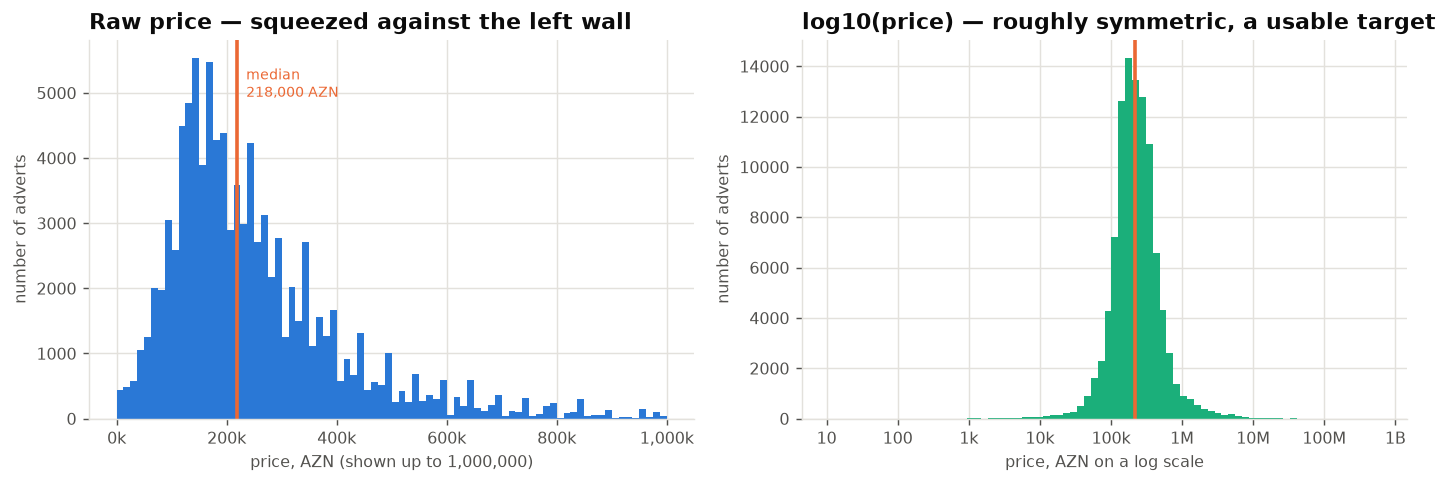
\includegraphics[width=0.92\textwidth]{price_distribution}
  \caption{The target before and after taking a logarithm. On the left,
  raw prices in AZN: the long tail of expensive properties stretches the
  axis so far that the ordinary market becomes a single spike. On the
  right, the same prices on a logarithmic scale, which is close to
  symmetric and is what we actually train on.}
  \label{fig:price}
\end{figure*}
% ---------------------------------------------------------------------

\section{The Four Real Problems}

Exploration is not a formality. Four problems in this dataset would each
have produced a model with excellent scores and no value.

\subsection{Problem 1: columns that contain the answer}

Three columns secretly carry the price.

\textbf{\texttt{total\_price}} is equal to \texttt{price} in
\textbf{99.99\%} of rows. It is the target wearing a different name.

\textbf{\texttt{unit\_price}} is the price per square metre. We checked
whether it rebuilds the price: multiplying it by the area recovers the
exact price on \textbf{100.0\%} of the 75{,}996 rows where both values
are present. It is the target divided by a column we keep.

\textbf{\texttt{description}} is free text written by the seller, and in
roughly 17\% of a sample it states the price in words.

A model trained with any of these would score almost perfectly and would
be useless, because in real life you do not know the price per square
metre of a flat before you know its price. All three are removed.

\subsection{Problem 2: the same property, many times}

Asking pandas for duplicate rows returns \textbf{zero}: no two rows are
identical across all 51 columns. The duplication is at a different level.

The file was scraped repeatedly between \textbf{5 October and 19 November
2024}. An advert still online on two scrape days appears twice, with a
different timestamp and a different view count. One advert appears up to
seventeen times. Counting adverts rather than rows, 100{,}775 rows
describe only about 63{,}000 distinct properties.

This matters because of how we test a model. We train on one part of the
data and measure on another part the model has never seen. If the same
flat sits in both parts, the model does not predict its price --- it
remembers it. The score would be high and meaningless.

\subsection{Problem 3: one column, two units}

The area column \texttt{Sahe} stores text such as
\texttt{``145 m$^2$''}. For six of the seven property types the unit is
square metres. For bare land it is \textbf{sot}, a local unit equal to
100~square metres.

Read the numbers and ignore the words, and a 12-sot plot (1{,}200~m$^2$)
becomes the number 12 --- five times \emph{smaller} than a 65~m$^2$ flat.
Nothing crashes and no warning appears. The model simply learns that
large plots of land are tiny.

\subsection{Problem 4: empty does not mean unknown}

Several columns are mostly empty: \texttt{vip} is 91.5\% empty,
\texttt{featured} 96.9\%, \texttt{mortgage} 67.3\%. A common rule of
thumb says to delete any column that is more than 70\% empty.

That rule would be wrong here. Each of these columns has exactly
\textbf{one} distinct non-empty value. The site only writes them down
when the answer is yes, and leaves the cell empty for no. An empty cell
is therefore an answer, not a gap. Fig.~\ref{fig:missing} marks these
columns in orange. Filling them with an average, or deleting their rows,
would throw away perfectly good information --- in the case of
\texttt{vip}, 91\% of the dataset.

% ---------------------------------------------------------------------
\begin{figure}[t]
  \centering
  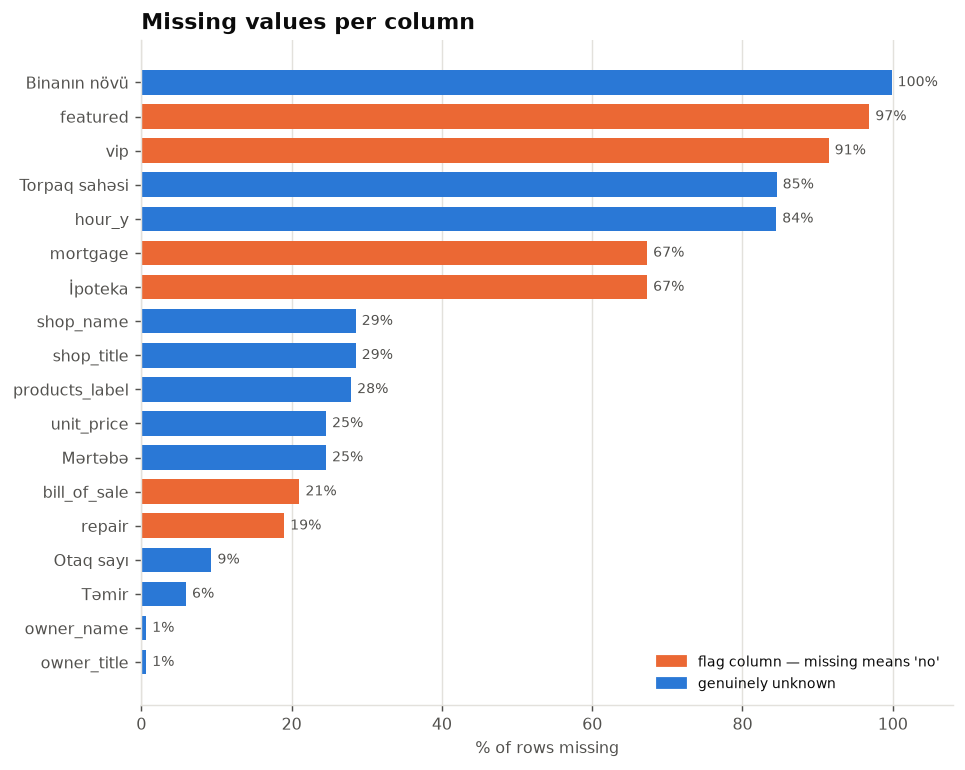
\includegraphics[width=\columnwidth]{missing_values}
  \caption{How much of each column is empty. Orange columns are the ones
  where an empty cell means ``no'' rather than ``unknown''; they are
  converted to 0/1 rather than filled in or dropped.}
  \label{fig:missing}
\end{figure}
% ---------------------------------------------------------------------

\section{Deciding What Belongs in the Task}

\texttt{Kateqoriya} splits the adverts into seven property types: new
buildings, old buildings, houses, bare land, commercial units, offices
and garages. We had to decide whether this is one prediction problem or
several. Two measurements answered it.

\textbf{The types do not share a feature set.} Fig.~\ref{fig:avail}
shows how often each feature is filled in. The floor number exists for
\textbf{100\%} of new and old building adverts and for \textbf{0\%} of
everything else. The room count is absent for land, commercial units and
garages. These are not gaps that imputation can repair: a plot of land
does not have a floor, and the question does not apply.

\textbf{Prices behave differently.} For flats, the price per square
metre is tightly grouped: the expensive end is only about 1.9 to 2.0
times the cheap end. For commercial units the same measure is 8.7 times,
because what a shop is worth depends on what it earns, and that is
nowhere in this dataset.

% ---------------------------------------------------------------------
\begin{figure}[t]
  \centering
  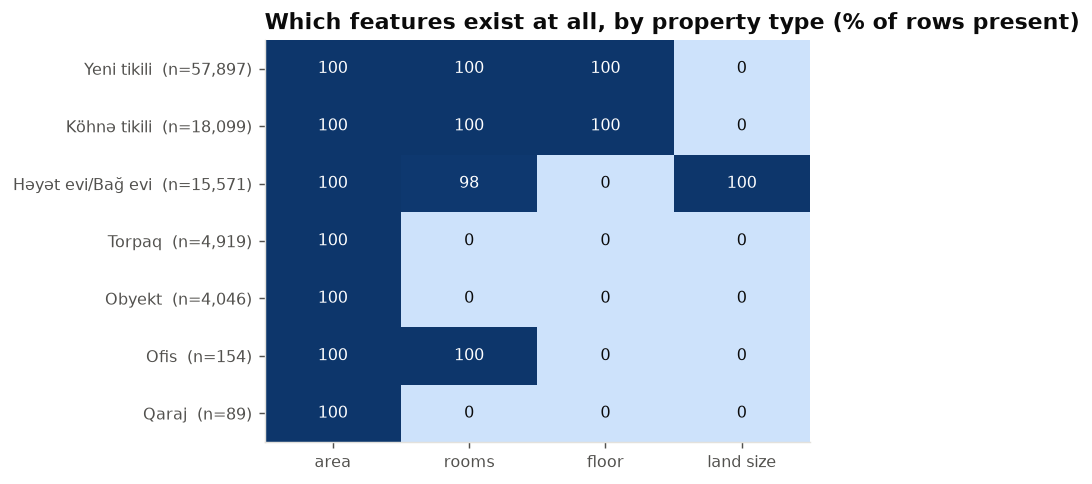
\includegraphics[width=\columnwidth]{feature_availability}
  \caption{Percentage of adverts where each feature is present, by
  property type. The floor number exists only for flats; land and
  commercial property record neither floor nor rooms. Mixing these types
  would leave most of the table structurally empty.}
  \label{fig:avail}
\end{figure}
% ---------------------------------------------------------------------

We therefore restrict the task to \textbf{residential property in Baku}:
new buildings, old buildings and houses. Baku accounts for 99.6\% of the
adverts in any case; the 260 adverts elsewhere are a different market
sampled too thinly to learn anything from. The property type is kept as
a feature, so the model can still tell a house from a new-build flat.

\section{The Preprocessing Steps}

The pipeline in \texttt{src/data\_prep.py} runs nine steps in order.
Table~\ref{tab:rows} records what each one costs in rows.

\subsection{Step 1--2: read and tidy}

We read the raw file and build a clean table from scratch, copying across
only the columns we intend to use. Numbers are pulled out of text:
\texttt{``145 m$^2$''} becomes 145, and \texttt{``7 / 9''} becomes floor~7
of a 9-storey building. Land measured in sot is converted to square
metres so that every area in the table uses one unit.

The yes/no columns are turned into 0 and 1. Three pairs of columns were
found to say exactly the same thing --- \texttt{repair} agrees with
\texttt{Temir} on 100.0\% of rows, and likewise for the
ownership certificate and the mortgage --- so one of each pair is kept.

Two columns are deliberately not used. \texttt{views} counts how many
people opened the advert, which is only known \emph{after} it is
published, so it cannot help price a property that is not yet listed.
\texttt{description} is free text and leaks the price.

\subsection{Step 3: one row per property}

Two passes, both before the data is split.

First, adverts are grouped by their page number and we keep the
\textbf{most recent sighting}. The choice is not arbitrary: among adverts
whose price moved between scrapes, it fell \textbf{2{,}606} times and
rose only \textbf{714}. Sellers cut prices that are not attracting
buyers, so the last sighting is the price the market saw last. This
removes 36{,}990 rows.

Second, a property is sometimes posted twice under two different advert
numbers. We find these by looking for adverts that agree on position,
size, room count \emph{and} price, and remove 544 more rows.

\subsection{Step 4--5: scope and impossible values}

The scope rule of Section~IV removes 6{,}172 adverts. Then four rules
remove records that cannot be true:

\begin{itemize}\itemsep2pt
  \item price outside \textbf{10{,}000--5{,}000{,}000~AZN};
  \item area outside \textbf{10--2{,}000~m$^2$};
  \item price per square metre outside \textbf{200--20{,}000~AZN};
  \item a flat on a floor higher than its own building.
\end{itemize}

The third rule earns its place. A 3-room flat listed at 73~AZN and a
200~m$^2$ flat listed at 600{,}000{,}000~AZN (three million AZN per square
metre) are typing mistakes, not bargains and not mansions. But price
alone is not enough: 12{,}000~AZN looks like a plausible cheap flat until
you notice it is 65~m$^2$, which works out at 185~AZN per square metre, far
below anything real. Together these rules remove only 66 adverts.

Two points of honesty. These are \textbf{fixed numbers written into the
code}, not percentiles measured from the data. A rule such as ``drop the
most expensive 1\%'' would let the test set influence what the training
set contains. And we \textbf{remove} these rows rather than pulling them
back to the nearest allowed value, because a 73~AZN flat is not an
extreme observation --- it is a broken record.

% ---------------------------------------------------------------------
\begin{table}[t]
  \centering
  \caption{What each cleaning step costs. Every number is written to
  \texttt{data/processed/preprocessing\_report.json} on each run.}
  \label{tab:rows}
  \small
  \begin{tabular}{@{}lrr@{}}
    \toprule
    Step & Rows removed & Rows left \\
    \midrule
    Raw file                       & ---     & 100{,}775 \\
    Repeat sightings of an advert  & 36{,}990 & 63{,}785 \\
    Property posted twice          & 544     & 63{,}241 \\
    Outside Baku / not residential & 6{,}172  & 57{,}069 \\
    Impossible values              & 66      & \textbf{57{,}003} \\
    \bottomrule
  \end{tabular}
\end{table}
% ---------------------------------------------------------------------

\subsection{Step 6: splitting, and why it comes here}

The data is shuffled once with a fixed random seed and cut
\textbf{70/15/15} into training, validation and test sets: 39{,}902,
8{,}550 and 8{,}551 properties.

The position of this step is the most important ordering decision in the
whole pipeline. Everything that is \emph{learned} from the data ---
which locations deserve a column, the values used to fill gaps, the
numbers used for scaling, the boundary between a cheap and an expensive
property --- is measured \textbf{after} this split and \textbf{only on
the training set}. If we had measured them first, information from the
test set would quietly reach the model and our final score would flatter
us.

Because Step~3 already guaranteed that each property appears exactly
once, a simple random split is safe: nothing can cross the boundary.

\subsection{Step 7--8: building the features}

Each property becomes \textbf{82 numbers}.

\textbf{Eleven continuous features}: floor area, land area, rooms, floor,
building height, latitude and longitude, plus the four engineered ones
described in Section~IV-F. The two areas are passed
through a logarithm first, because floor area and price form almost a
straight line once both are logged --- which is exactly the shape a
straight-line model can use. All seven are then rescaled to have an
average of 0 and a spread of 1, using the average and spread
\emph{of the training set}. This matters for the SVM, where an area in
the hundreds would otherwise drown out a 0/1 flag; the decision tree is
unaffected either way.

\textbf{Nine yes/no features}: renovated, ownership certificate,
mortgage available, promoted listing, featured listing, sold by the owner
rather than an agency, whether the floor number exists at all, and whether
the flat is on the ground or the top floor.

That last one deserves a note. Houses have no floor number, and filling
it with a typical value would invent a fifth floor for a bungalow.
Instead we store 0 and raise a flag saying ``this number is not real'',
which lets the model learn to ignore the floor columns for houses.

\textbf{Sixty-two yes/no columns for the categories}: three for the
property type, and 59 for location. Location is the strongest categorical
feature we have --- across the twenty most common districts the typical
price varies by a factor of 4.3, and Fig.~\ref{fig:map} shows the same
pattern geographically, with expensive property concentrated around the
bay and fading outwards. There are 142 district names in total, so we
give a column only to those appearing at least 100 times in the training
set and put the rest into a shared ``other'' column. This also means an
unfamiliar district appearing later cannot break anything.

% ---------------------------------------------------------------------
\begin{figure}[t]
  \centering
  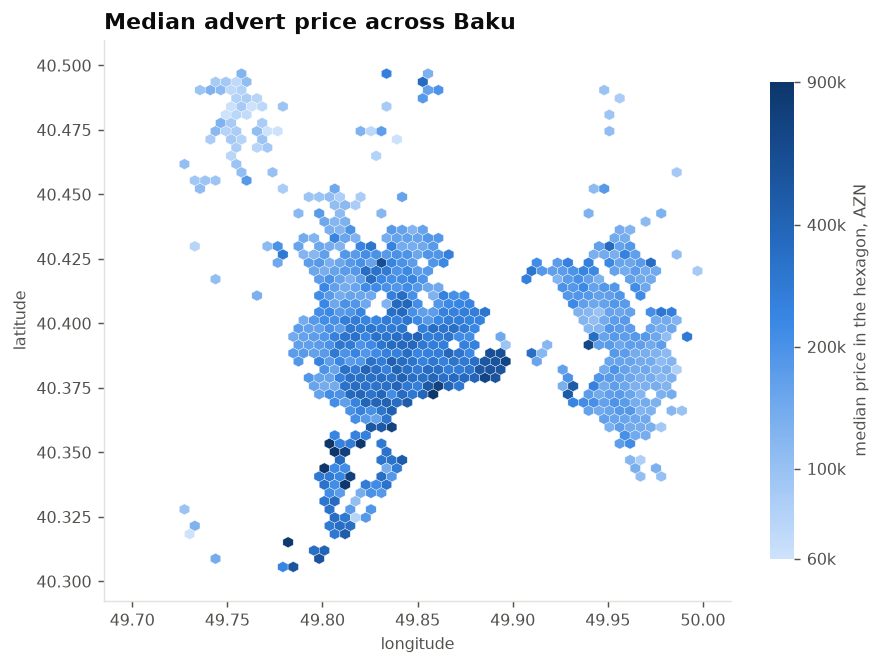
\includegraphics[width=\columnwidth]{map_of_baku}
  \caption{Typical advert price across Baku. The city is divided into
  small hexagons and each is shaded by the middle price of the adverts
  inside it. The smooth gradient from the centre outwards is why
  coordinates are worth keeping as features.}
  \label{fig:map}
\end{figure}
% ---------------------------------------------------------------------

\subsection{Feature engineering: four things the columns imply
but never state}

Everything described so far either cleans a value or rewrites it in a form
a model can read. None of it adds an idea. Four of the features do.

They contain no new information --- each is computed from columns we
already have. What they add is \emph{shape}. A straight-line model such as
an SVM can only multiply each input by a weight and add the results up; it
cannot divide one input by another, and it cannot measure a distance. A
decision tree can imitate these by stacking many splits, but it has to
spend depth doing so. Writing them out as columns hands both models the
relationship directly.

\textbf{1. Distance from the centre of Baku.} The price map
(Fig.~\ref{fig:map}) shows a smooth fade from the bay outwards, but a
model given only latitude and longitude sees two numbers that mean nothing
on their own. We measure the straight-line distance in kilometres from
Icherisheher, the old walled city. That landmark is a fixed coordinate
written into the code, not a value measured from the data, so it cannot
shift between runs.

\textbf{2. How high up the building the flat sits}, as a fraction from 0
to 1. Floor 3 means something different in a 4-storey building than in a
20-storey one, and the raw floor number cannot say which. We add two
further flags for the floors buyers react to: the ground floor, and the
top floor.

\textbf{3. Average room size}, the floor area divided by the room count.
Two 90~m$^2$ flats, one with two rooms and one with four, are different
products. Size alone does not separate them and room count alone does not
either; the ratio does.

\textbf{4. How much land comes with the building}, relative to the
building itself. The same house on a larger plot is worth more. Flats
have no land, so this is zero for them.

Measured against the price, the average room size turns out to be the
\textbf{second strongest feature in the whole set}, behind only the floor
area itself. Distance from the centre ranks ninth, ahead of every
individual district column.

Table~\ref{tab:fe} shows what the four are worth. We trained the same
reference models on the data with and without them. The gain is real but
modest, and --- against our expectation --- it is the \emph{shallow}
decision tree that benefits most, not the straight-line model. The reason
is instructive: a shallow tree has only a few splits to spend, so being
handed a ratio outright saves it work it could not otherwise afford.

% ---------------------------------------------------------------------
\begin{table}[t]
  \centering
  \caption{What the four engineered features are worth. Scores are
  $R^2$ on the validation set for Task~A, same data, same seeds, with
  only the six extra columns differing.}
  \label{tab:fe}
  \small
  \begin{tabular}{@{}lccc@{}}
    \toprule
    Reference model & 76 features & 82 features & Gain \\
    \midrule
    Straight line (ridge)   & 0.8498 & 0.8550 & $+0.0051$ \\
    Decision tree, depth 8  & 0.8277 & 0.8403 & $+0.0127$ \\
    Decision tree, depth 13 & 0.8520 & 0.8560 & $+0.0040$ \\
    \bottomrule
  \end{tabular}
\end{table}
% ---------------------------------------------------------------------

We stopped at four. Every added column is one more thing the report has to
justify, and two tempting ideas were rejected outright. Replacing each
district with its average price would push the target into a feature and
leak. Adding the price per square metre, which is the strongest predictor
imaginable, would leak completely --- it is the target divided by a column
we keep, and Section~II-A is the reason we deleted it in the first place.

\subsection{The two targets}

\textbf{Task A} predicts the \textbf{logarithm} of the price rather than
the price itself. Prices here span six orders of magnitude. Measured in
manat, one mistake on a 5{,}000{,}000~AZN property outweighs thousands of
mistakes on ordinary flats, so the model would spend all its effort on a
handful of mansions. A logarithm turns ``twice as expensive'' into a
fixed step, which is how people actually compare properties.

\textbf{Task B} predicts whether a property is \emph{premium} or
\emph{standard}, split at the middle price of the \textbf{training set},
which is \textbf{209{,}000~AZN}. Using the middle price of the whole
dataset would let test prices decide the boundary, which is the same
leak in a different disguise. Prices cluster on round numbers, so 117
training properties sit exactly on the boundary; counting them as
premium gives a 50.01/49.99 split instead of 49.71/50.29.

\section{Checking the Result}

A preprocessing pipeline that is only inspected by eye is not evidence.
\texttt{src/validate.py} re-reads the output and runs \textbf{58
automatic checks}, all of which pass. Among them:

\begin{itemize}\itemsep2pt
  \item no property appears in more than one of the three sets;
  \item the three sets really are 70/15/15 and add up to the total;
  \item the stored targets match the prices in the readable tables;
  \item the premium boundary equals the training-set middle price;
  \item no feature contains a missing or infinite value;
  \item no column is suspiciously close to the price, which would
        indicate a leak we had missed;
  \item running the whole pipeline a second time produces
        \textbf{identical} sets, verified by comparing fingerprints of
        the property identifiers.
\end{itemize}

As a final sanity check, we fitted off-the-shelf reference models to the
prepared data. They reach an $R^2$ of 0.856 on Task~A and 92.3\%
accuracy on Task~B. These numbers are useful precisely because they are good but
not perfect: a near-perfect score would have told us that a leak was
still present.

\section{Summary}

The raw file was 100{,}775 adverts and 51 columns. After removing
repeated sightings, restricting the task to Baku residential property,
and deleting records that cannot be true, \textbf{57{,}003 properties}
remain, each described by \textbf{82 features}.

The work that mattered was not complicated. It was reading the columns
carefully enough to notice that one of them changes unit halfway down,
that another is the answer in disguise, that an empty cell sometimes
means ``no'', and that the same flat can appear seventeen times. Each of
these is invisible to a program that simply loads the file and starts
training, and each would have produced a model that scores well and
predicts nothing.

Every number in this report is regenerated by
\texttt{python -m src.run\_all} from a clean checkout.

\end{document}
